\documentclass[10pt,a4paper]{article}
\usepackage[latin1]{inputenc}
\usepackage{amsmath}
\usepackage{amsfonts}
\usepackage{amssymb}
\usepackage{graphicx}

\begin{document}
\section*{Solving Helmholtz For A House}
We constructed a house which was 8 x 6 meters large. The simple, yet delicate interior consisted of a circular swimming pool in the middle of the house, as well as an exquisite box made of teflon in one of the corners. The outer walls were made of wood. The house plan is given in figure \ref{fig:housePlan}. The constants we used for permittivity and permeability for each material is given in \cite{dielectric}.

\begin{figure}[h]
\centering
    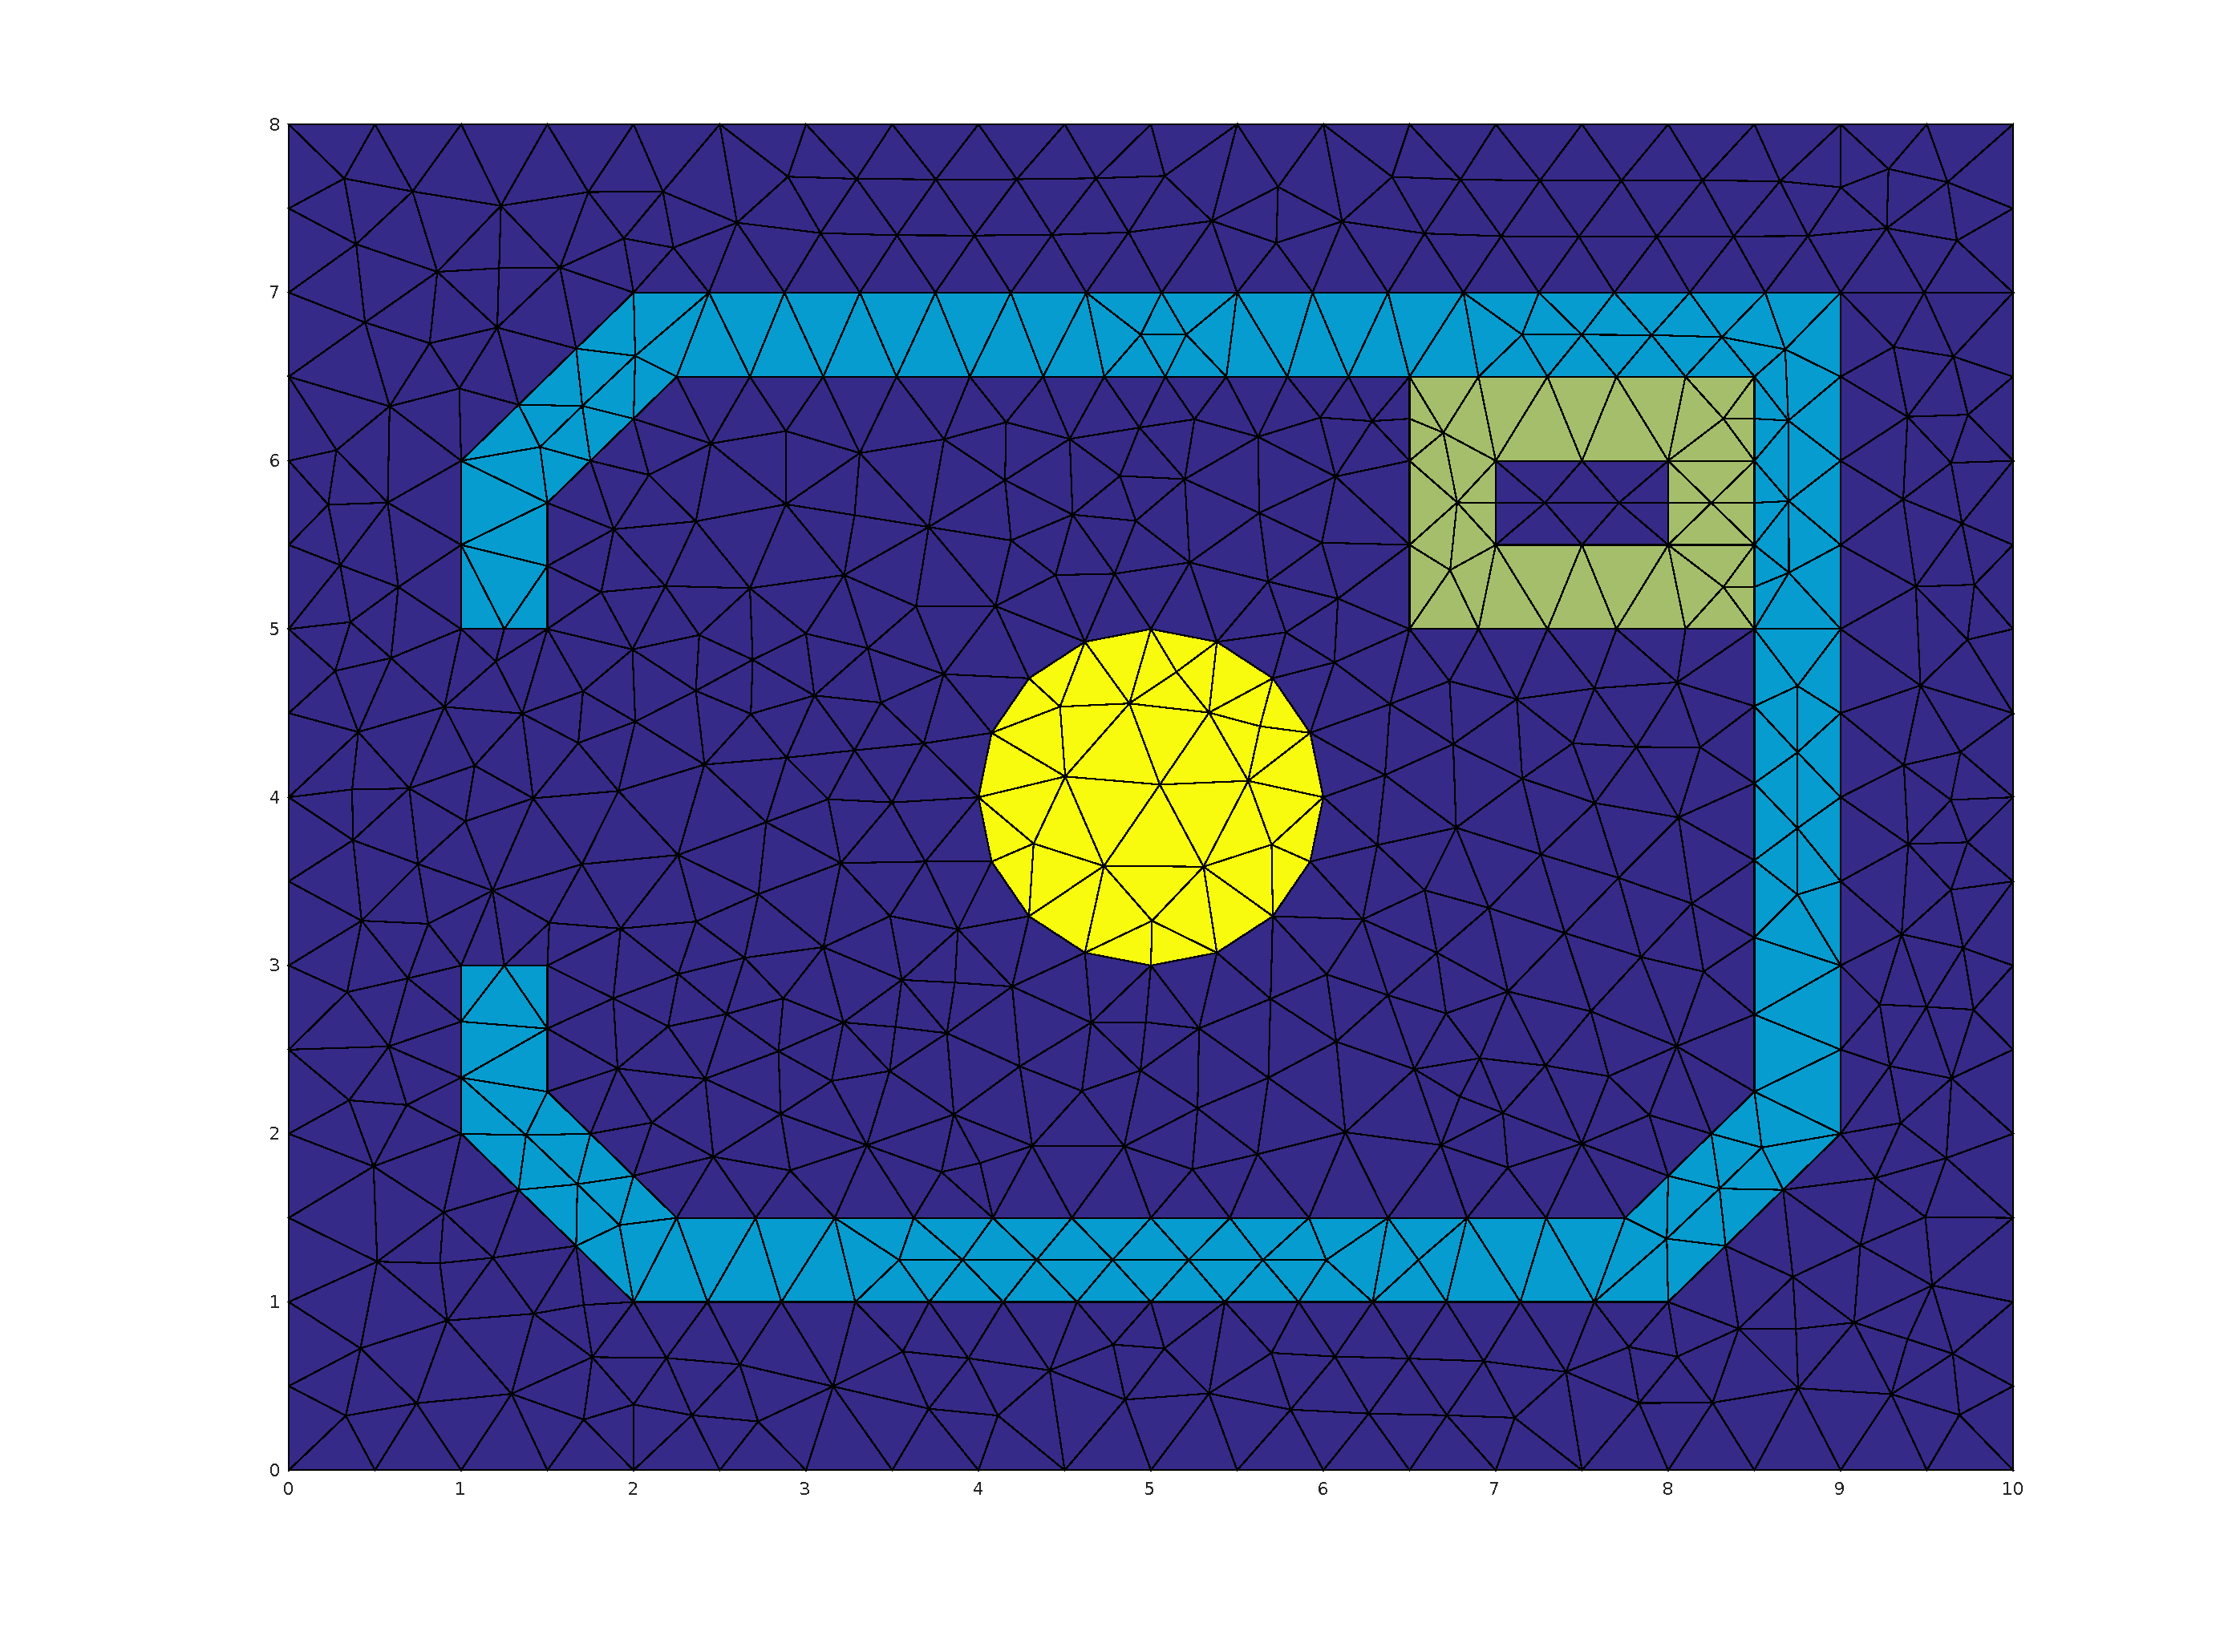
\includegraphics[width=0.9\textwidth]{figures/geometry.pdf}
	\caption{A domain which illustrates a house. The yellow disc is water, the turquoise section is the wall, while the green part in the corner is a box made of teflon.}
  \label{fig:housePlan}
\end{figure}

For the solution of Helmholtz in the house domain we used Robin boundary conditions, with a maximum diameter for the triangles equal to 0.05, i.e. $h = 0.05$. A complex $k$ gave an attenuated signal. We wanted to check how the shapes with differing materials in the domain affected the intensity of our signal. Initially we placed one source in the top left of the house. The result is seen in figure \ref{fig:house1source}. We also wanted to see how the intensity changed when we added an additional source. The source was placed in the bottom right corner of the house. This can be seen in figure \ref{fig:house2sources}. 

For both cases we saw that the swimming pool with water resulted in close to zero intensity for the signal. This was also the case for the teflon box. EM-signals were effectively stopped in both materials. We also realized that the EM-waves propagated better in wood compared to air, which is why we see the signal strength increasing in these regions.

When the second source is introduced in figure \ref{fig:house2sources} we can also see that we get interference in the signal.

\begin{figure}[H]
\centering
    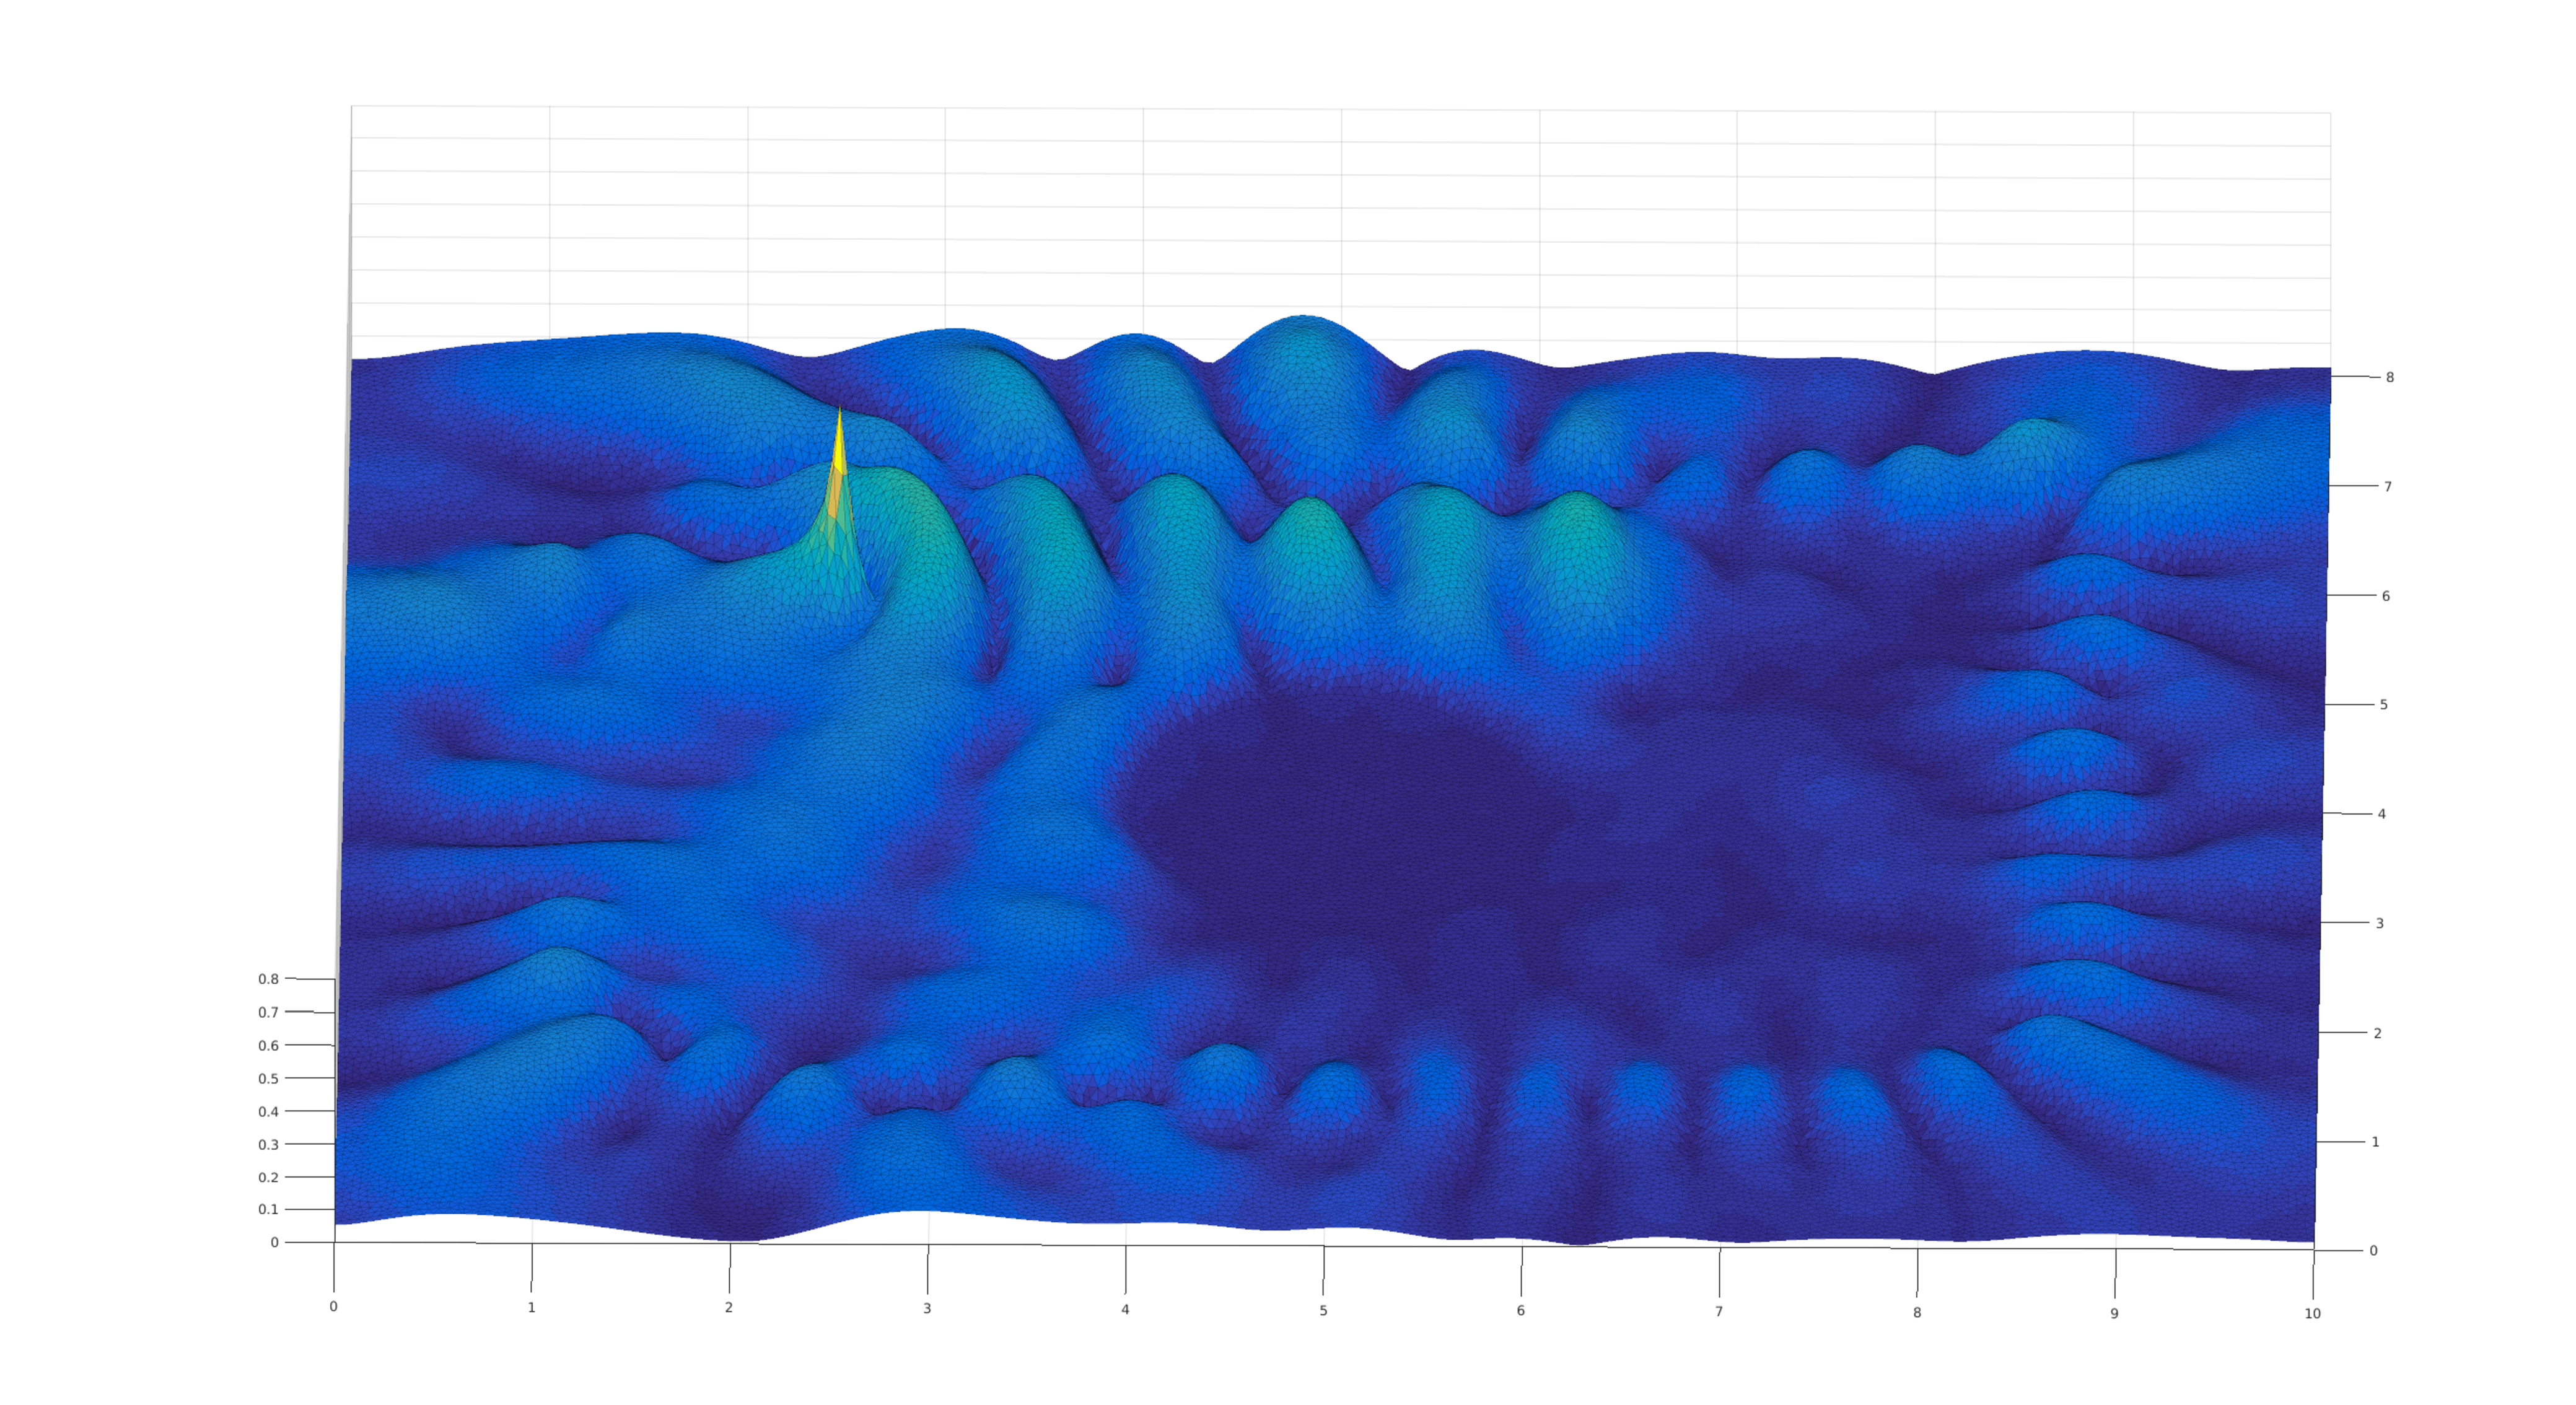
\includegraphics[width=0.9\textwidth]{figures/house_topleft_source.pdf}
	\caption{One point source with Robin boundary conditions. Maximum diameter $h$ of a triangle is equal to 0.05. }
  \label{fig:house1source}
\end{figure}

\begin{figure}[H]
\centering
    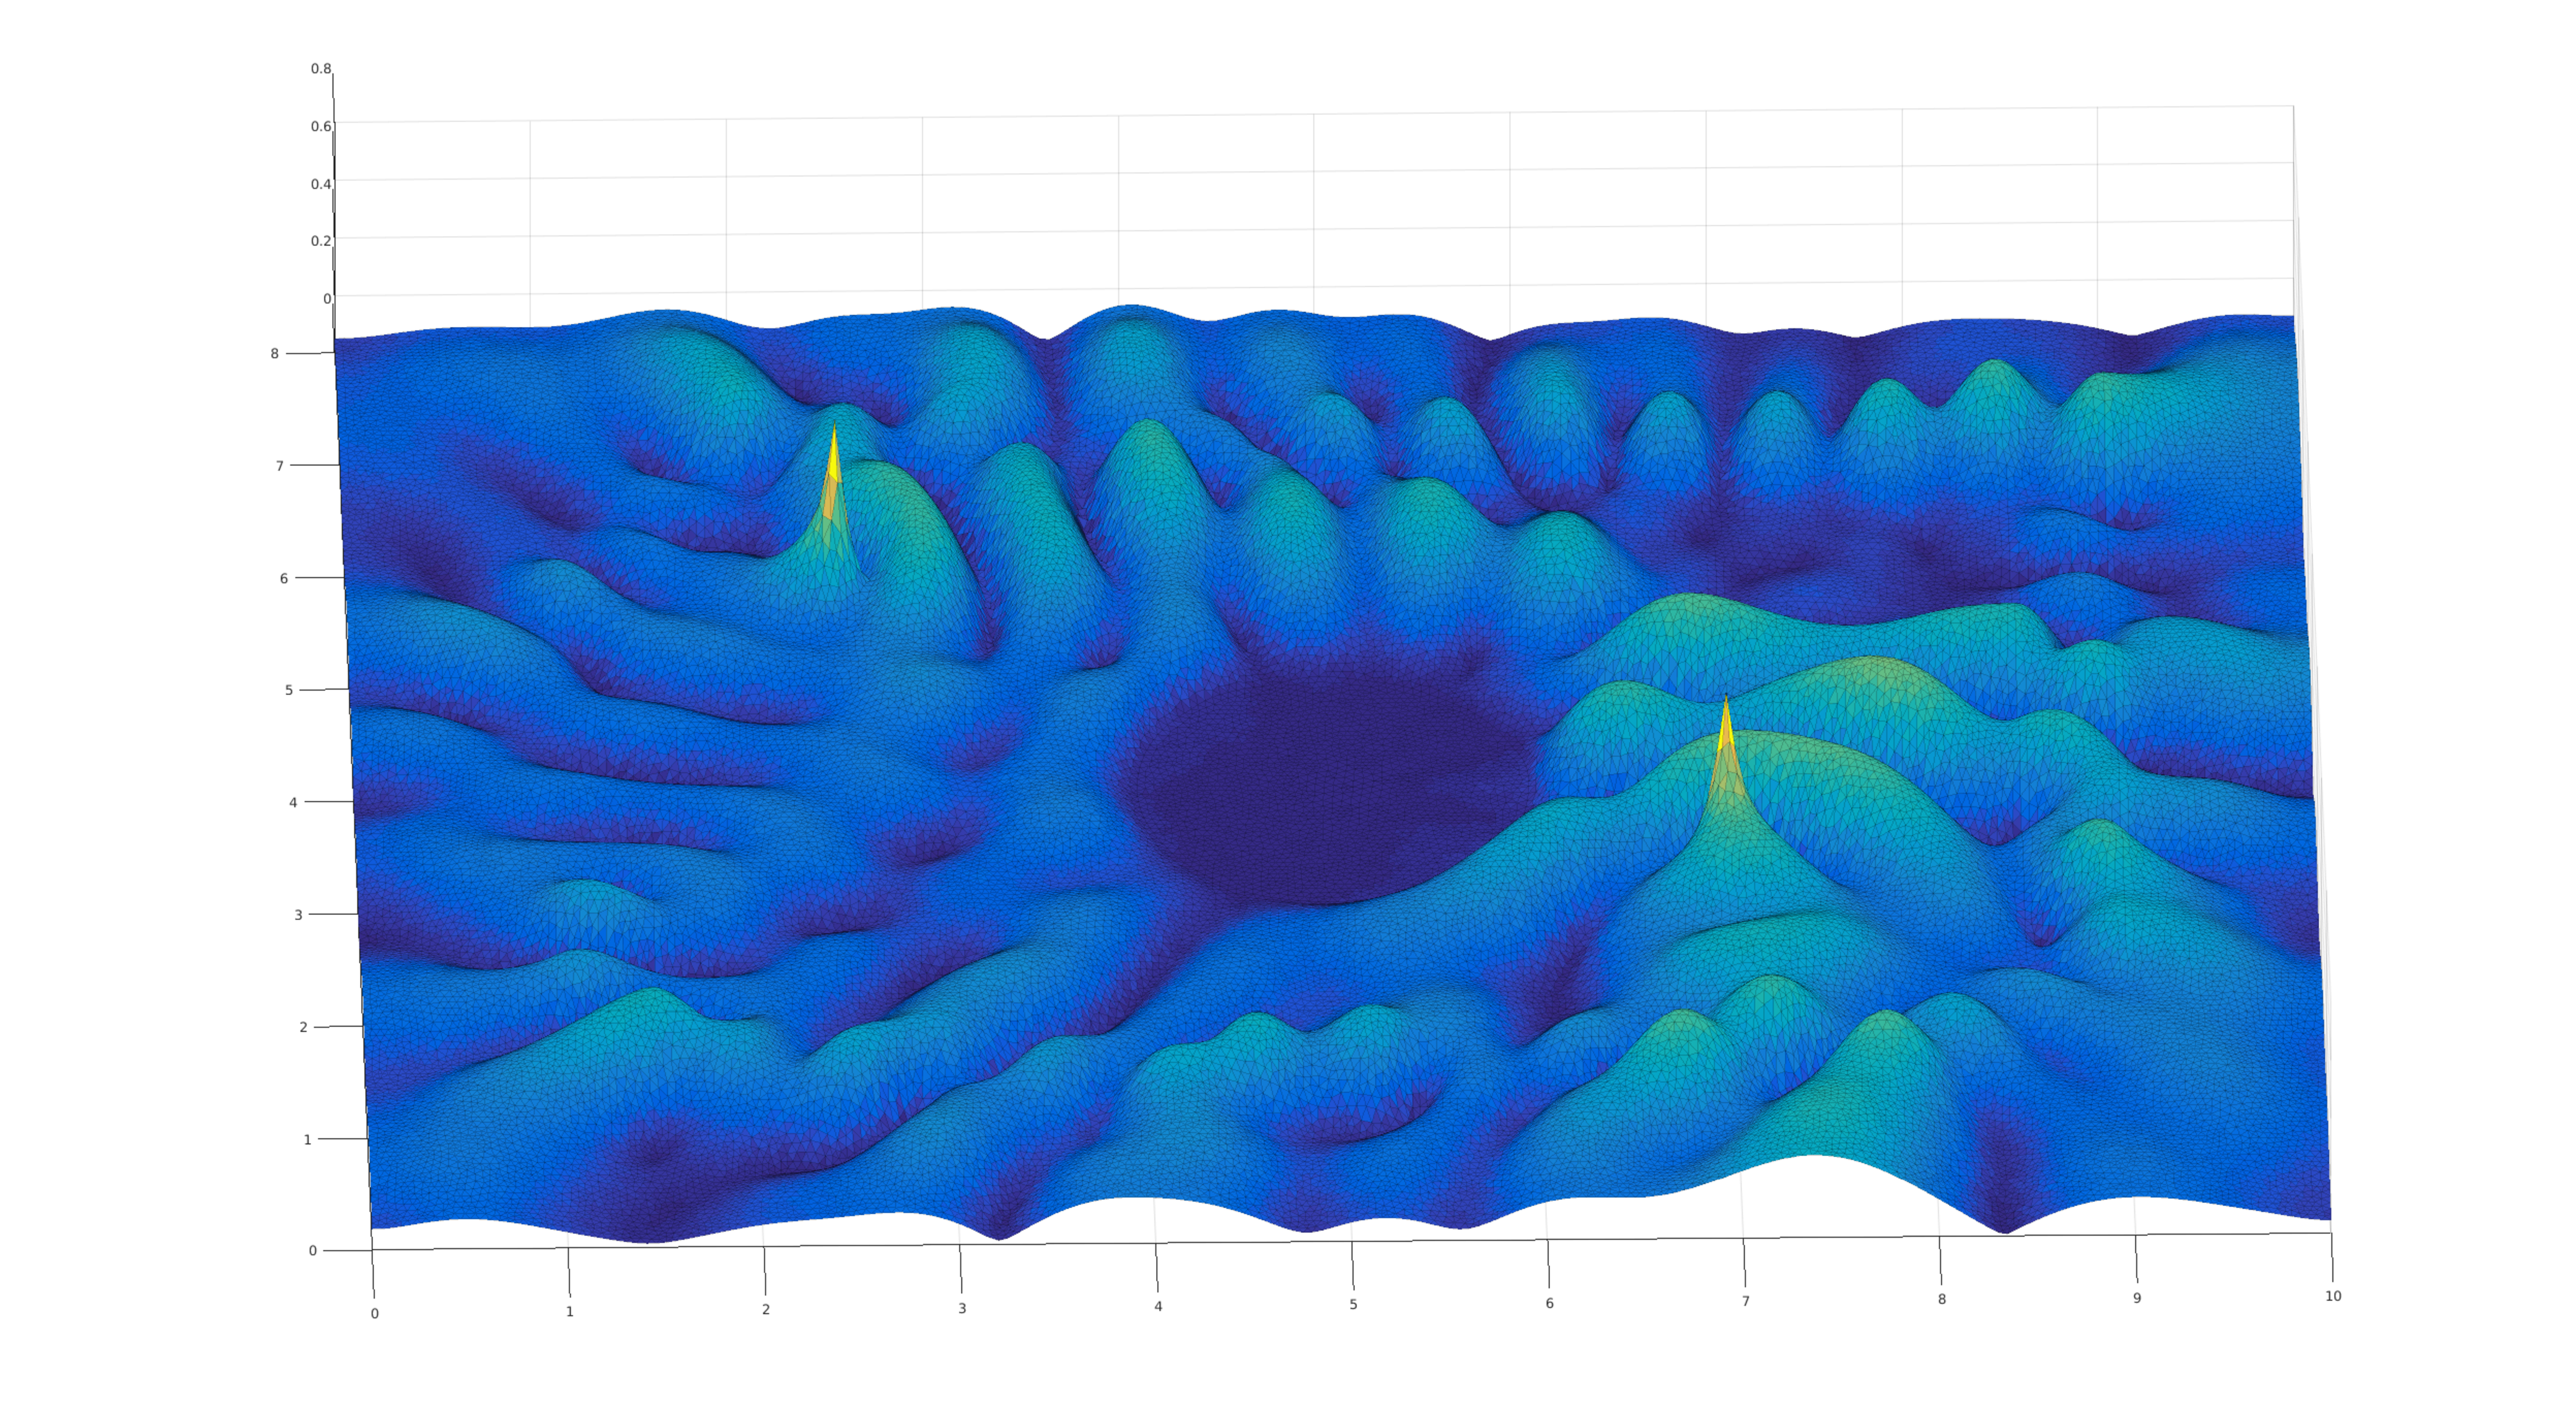
\includegraphics[width=0.9\textwidth]{figures/house_doublesource.pdf}
	\caption{Two point sources with Robin boundary conditions in the house. $h$ is equal to 0.05.}
  \label{fig:house2sources}
\end{figure}



\end{document}